% =====================================================================
% Capítulo: Propuesta (AST-CC)
% =====================================================================

\chapter{AST-CC: refinamiento jerárquico de ST-CC guiado por pruebas de hipótesis}\label{chap:propuesta}

Este capítulo presenta el método propuesto, al que se denomina \emph{Adaptive
Spatio-Temporal Co-Clustering} (AST-CC). El método conserva la partición en
tablero que produce ST-CC y la toma como punto de partida de un árbol de
refinamientos locales: cada bloque se examina por separado y, si contiene
interacción residual entre regiones y horarios que sea estadísticamente
detectable y de tamaño relevante, se subdivide; en caso contrario, se conserva
como hoja.

El capítulo sigue el mismo orden lógico que el anterior, de lo general a lo
específico. Primero se da una visión general del método. Luego se formaliza el
refinamiento como un árbol de bloques y se demuestra que la función objetivo se
descompone de forma exacta por hojas, lo que convierte la ganancia de cada corte
en un estadístico de razón de verosimilitud. Sobre esa base se definen los
estadísticos de heterogeneidad, la regla de decisión, la calibración de las
pruebas, el control de comparaciones múltiples y los criterios de parada. El
capítulo termina con el algoritmo completo, su costo computacional, la forma de
presentar los resultados y las limitaciones del diseño.

\section{Visión general}\label{sec:prop-vision}

La idea central de AST-CC puede resumirse en una frase: \emph{refinar mientras
haya heterogeneidad local estadísticamente detectable y de tamaño relevante, y
detenerse cuando todas las hojas sean indistinguibles de su modelo nulo local}.
Es la traducción al objeto bidimensional del principio de SigTree
\cite{Hu2025}, que detiene el crecimiento de su árbol cuando ninguna división
candidata es significativa.

El método se organiza en cuatro etapas, que se ilustran en la
Figura~\ref{fig:prop-teselacion}:

\begin{enumerate}
  \item \textbf{Construcción de la matriz.} Los viajes se agregan en una
  matriz $O \in \mathbb{N}^{m\times n}$ de conteos totales región $\times$
  intervalo de tiempo. Se usan conteos y no promedios diarios, por la razón
  expuesta en la Sección~\ref{sec:escala}: solo sobre conteos la
  I-divergencia coincide con la devianza de Poisson.
  \item \textbf{Partición base.} Se ejecuta BBAC$_I$ con $K_R$ grupos de
  filas y $K_T$ grupos de columnas, con la base C5 adoptada en la
  Sección~\ref{sec:stcc-base} (la base C2 se conserva como variante). El
  resultado es exactamente la partición de ST-CC.
  \item \textbf{Refinamiento.} Cada uno de los $K_R K_T$ bloques se somete a
  un procedimiento recursivo que decide, mediante pruebas de hipótesis, si se
  divide por filas, por columnas, de forma conjunta, o si se convierte en hoja.
  \item \textbf{Resumen.} Las hojas del árbol se describen con su tamaño de
  efecto y su nivel de actividad relativo, y se representan de forma que se
  conserve la lectura espacial y temporal que ofrece ST-CC.
\end{enumerate}

\begin{figure}[t]
\centering
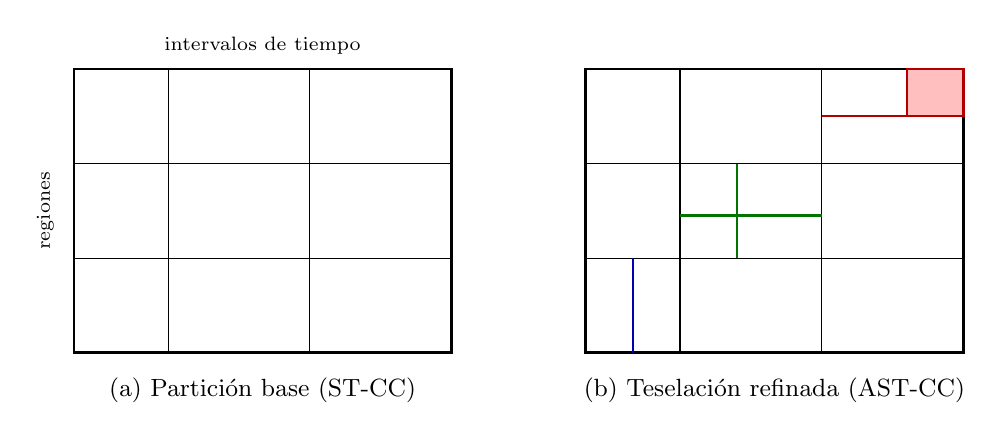
\begin{tikzpicture}[x=0.6cm,y=0.6cm]
  % ---- Panel izquierdo: tablero de ST-CC ----
  \begin{scope}
    \draw[thick] (0,0) rectangle (8,6);
    \foreach \x in {2,5} \draw (\x,0) -- (\x,6);
    \foreach \y in {2,4} \draw (0,\y) -- (8,\y);
    \node at (4,-0.8) {\small (a) Partición base (ST-CC)};
    \node[rotate=90] at (-0.6,3) {\scriptsize regiones};
    \node at (4,6.5) {\scriptsize intervalos de tiempo};
  \end{scope}
  % ---- Panel derecho: teselación refinada ----
  \begin{scope}[xshift=6.5cm]
    \draw[thick] (0,0) rectangle (8,6);
    \foreach \x in {2,5} \draw (\x,0) -- (\x,6);
    \foreach \y in {2,4} \draw (0,\y) -- (8,\y);
    % bloque (fila 1, col 3): corte de filas y luego corte de columnas
    \draw[red!70!black, thick] (5,5) -- (8,5);
    \draw[red!70!black, thick] (6.8,5) -- (6.8,6);
    \fill[red!25] (6.8,5) rectangle (8,6);
    \draw[red!70!black, thick] (6.8,5) rectangle (8,6);
    % bloque (fila 3, col 1): corte de columnas
    \draw[blue!70!black, thick] (1,0) -- (1,2);
    % bloque (fila 2, col 2): corte conjunto 2x2
    \draw[green!45!black, thick] (3.2,2) -- (3.2,4);
    \draw[green!45!black, thick] (2,2.9) -- (5,2.9);
    \node at (4,-0.8) {\small (b) Teselación refinada (AST-CC)};
  \end{scope}
\end{tikzpicture}
\caption{Comparación entre la partición en tablero de ST-CC y la teselación que
produce AST-CC. En (b), un bloque se refinó con un corte de filas seguido de un
corte de columnas (rojo; la hoja sombreada representa un patrón local), otro con
un corte de columnas (azul) y otro con un corte conjunto $2\times 2$ (verde).
Los cortes solo afectan al bloque en que se producen, por lo que el resultado
deja de ser una rejilla global.}
\label{fig:prop-teselacion}
\end{figure}

La diferencia con aumentar $K_R$ y $K_T$ es visible en la figura: en una
rejilla global, cada nuevo corte atraviesa toda la matriz; en AST-CC, afecta
solo al bloque donde se detectó la heterogeneidad.

\section{Formulación del refinamiento}\label{sec:prop-formulacion}

\subsection{Notación}

Se mantiene la notación del Capítulo~\ref{chap:marco}. Un \emph{bloque} es un
producto $B = I \times J$ con $I \subseteq \{1,\dots,m\}$ y
$J \subseteq \{1,\dots,n\}$. Para un bloque se definen sus totales internos
\[
  O^{B}_{i\cdot} = \sum_{j\in J} O_{ij}\ (i\in I), \qquad
  O^{B}_{\cdot j} = \sum_{i\in I} O_{ij}\ (j\in J), \qquad
  N_B = \sum_{(i,j)\in B} O_{ij},
\]
y los conteos esperados bajo independencia entre filas y columnas dentro del
bloque,
\begin{equation}\label{eq:prop-EB}
  E^{B}_{ij} = \frac{O^{B}_{i\cdot}\, O^{B}_{\cdot j}}{N_B},
  \qquad (i,j)\in B .
\end{equation}
El estadístico de razón de verosimilitud de la prueba de independencia en el
bloque y la información mutua empírica asociada son, como en
\eqref{eq:c6-g2} y \eqref{eq:g2-im},
\begin{equation}\label{eq:prop-G2}
  G^2_B = 2\sum_{(i,j)\in B} O_{ij}\log\frac{O_{ij}}{E^{B}_{ij}},
  \qquad
  \hat I_B = \frac{G^2_B}{2N_B}.
\end{equation}
La cantidad $\hat I_B$ se mide en \emph{nats por observación}, no depende del
tamaño de la muestra y se usará como tamaño de efecto.

\subsection{Árbol de bloques y teselación guillotina}

El objeto que optimiza AST-CC deja de ser un par de mapeos $(\rho,\tau)$ y pasa
a ser un árbol de bloques anidados.

\begin{definicion}[Corte de un bloque]\label{def:corte}
Un \emph{corte} $s$ de un bloque $B = I\times J$ es una partición de $B$ en
bloques hijos de uno de tres tipos:
\begin{enumerate}
  \item \emph{de filas}: $\{I_1\times J,\ I_2\times J\}$, con
  $\{I_1,I_2\}$ partición de $I$;
  \item \emph{de columnas}: $\{I\times J_1,\ I\times J_2\}$, con
  $\{J_1,J_2\}$ partición de $J$;
  \item \emph{conjunto}: $\{I_a\times J_b\}_{a,b\in\{1,2\}}$, con
  $\{I_1,I_2\}$ y $\{J_1,J_2\}$ particiones de $I$ y de $J$.
\end{enumerate}
Se denota $\mathcal{C}(B,s)$ al conjunto de hijos.
\end{definicion}

\begin{definicion}[Árbol de refinamiento]\label{def:arbol}
Un \emph{árbol de refinamiento} $\mathcal{T}$ es un árbol con raíz en el que
\begin{enumerate}
  \item los hijos de la raíz son los $K_R K_T$ bloques
  $B_{gh} = I_g\times J_h$ de la partición base $(\rho,\tau)$;
  \item cada nodo interno $B$ tiene como hijos los bloques
  $\mathcal{C}(B,s_B)$ de un corte $s_B$.
\end{enumerate}
El conjunto de hojas se denota $\mathcal{L}(\mathcal{T})$.
\end{definicion}

Por construcción, $\mathcal{L}(\mathcal{T})$ es una partición de
$\{1,\dots,m\}\times\{1,\dots,n\}$ en rectángulos (en el sentido de
subconjuntos de filas por subconjuntos de columnas) con estructura de
guillotina anidada. Cuando el árbol no tiene nodos internos por debajo de la
partición base, $\mathcal{L}(\mathcal{T})$ coincide con el tablero de ST-CC.
Dos filas que pertenecen al mismo grupo base pueden terminar en hojas con
particiones temporales distintas; esta es precisamente la flexibilidad que se
busca.

\subsection{Modelo local y aproximación}

A cada árbol se le asocia una aproximación de la matriz. La elección coherente
con el Capítulo~\ref{chap:marco} es modelar cada hoja con el modelo de
independencia de su propio bloque.

\begin{definicion}[Aproximación de un árbol]\label{def:aprox-arbol}
Para $(i,j)$, sea $L(i,j)\in\mathcal{L}(\mathcal{T})$ la hoja que la contiene.
La aproximación asociada a $\mathcal{T}$ es
\[
  \hat O^{\mathcal{T}}_{ij} = E^{L(i,j)}_{ij}
  = \frac{O^{L}_{i\cdot}\, O^{L}_{\cdot j}}{N_L}\,,\qquad L = L(i,j).
\]
\end{definicion}

Cuando las hojas son los bloques base, $\hat O^{\mathcal{T}}$ es la
aproximación de la base C6 \cite{Banerjee2007} para la partición $(\rho,\tau)$.
En general, $\hat O^{\mathcal{T}}$ es el estimador de máxima verosimilitud de un
modelo log-lineal de Poisson en el que cada hoja tiene sus propios efectos de
fila y de columna, con $\sum_{L}(|I_L|+|J_L|-1)$ parámetros libres.

\subsection{Descomposición por hojas y ganancia de un corte}\label{sec:prop-descomp}

El siguiente resultado es la pieza que hace viable el esquema recursivo: la
divergencia del árbol se reparte exactamente entre sus hojas, y la reducción que
produce un corte es un estadístico de razón de verosimilitud que puede evaluarse
localmente.

\begin{proposicion}[Descomposición por hojas y ganancia de un corte]\label{prop:ganancia}
Sea $\mathcal{T}$ un árbol de refinamiento y supóngase que $E^{B}_{ij}>0$
siempre que $O_{ij}>0$.
\begin{enumerate}
  \item[(a)] La divergencia del árbol se descompone por hojas:
  \begin{equation}\label{eq:prop-desc-hojas}
    D_I\bigl(O \,\|\, \hat O^{\mathcal{T}}\bigr)
    = \frac12 \sum_{L\in\mathcal{L}(\mathcal{T})} G^2_L .
  \end{equation}
  \item[(b)] Si un bloque $B$ se divide mediante un corte $s$, entonces
  \begin{equation}\label{eq:prop-cadena}
    G^2_B = G^2_{B,s} + \sum_{C\in\mathcal{C}(B,s)} G^2_C ,
  \end{equation}
  donde $G^2_{B,s}\ge 0$ es el estadístico de razón de verosimilitud que
  compara la independencia en $B$ con el modelo en que cada hijo tiene sus
  propios efectos de fila y columna. Para un corte de filas
  $\{I_1, I_2\}$, con $O_{rj} = \sum_{i\in I_r} O_{ij}$ y
  $N_r = \sum_{j\in J} O_{rj}$,
  \begin{equation}\label{eq:prop-G2-colapsada}
    G^2_{B,s} = 2\sum_{r=1}^{2}\sum_{j\in J} O_{rj}
      \log\frac{O_{rj}\,N_B}{N_r\,O^{B}_{\cdot j}},
  \end{equation}
  que es el estadístico $G^2$ de independencia de la tabla colapsada
  $2\times|J|$. El caso de columnas es simétrico. Los grados de libertad
  asintóticos de $G^2_{B,s}$ son $|J|-1$ para un corte de filas, $|I|-1$
  para uno de columnas y $|I|+|J|-3$ para uno conjunto.
  \item[(c)] En consecuencia, sustituir la hoja $B$ por sus hijos reduce la
  divergencia del árbol exactamente en $\tfrac12\, G^2_{B,s}$.
\end{enumerate}
\end{proposicion}

\begin{proof}
(a) Dentro de cada hoja, la aproximación reproduce el total $N_L$, de modo que
$\sum_{(i,j)\in L}(O_{ij}-E^{L}_{ij}) = 0$ y los términos lineales de la
I-divergencia se cancelan. Queda
$\sum_{(i,j)\in L} d_I(O_{ij},E^L_{ij}) = \sum_{(i,j)\in L} O_{ij}\log(O_{ij}/E^L_{ij}) = \tfrac12 G^2_L$,
y basta sumar sobre las hojas.

(b) Restringido a $B$, el modelo de independencia,
$\log\mu_{ij} = \alpha_i + \beta_j$, está anidado en el modelo del corte. Para
un corte de filas, este último es $\log\mu_{ij} = \alpha_i + \beta_{r(i),j}$,
donde $r(i)$ indica el hijo de la fila $i$; para uno conjunto, es
$\log\mu_{ij} = \alpha_{i,b(j)} + \beta_{a(i),j}$, que es la base C6 restringida
al bloque. En los tres casos, la estimación de máxima verosimilitud del modelo
del corte coincide, sobre cada hijo $C$, con su aproximación de independencia
$E^{C}$. La identidad pitagórica usada en la demostración de la
Proposición~\ref{prop:descomposicion}, aplicada al par de modelos anidados,
da
\[
  D_I(O|_B \,\|\, E^{B})
  = \sum_{C\in\mathcal{C}(B,s)} D_I(O|_C \,\|\, E^{C})
  + D_I(\hat E^{B,s} \,\|\, E^{B}),
\]
donde $\hat E^{B,s}$ es la aproximación del modelo del corte. Multiplicando por
dos y usando (a) se obtiene \eqref{eq:prop-cadena} con
$G^2_{B,s} = 2D_I(\hat E^{B,s}\|E^B)$. Para un corte de filas, los totales de
fila de cada hijo coinciden con los de $B$, y
$\log(E^{C_r}_{ij}/E^{B}_{ij}) = \log\bigl(O_{rj}N_B/(N_r O^B_{\cdot j})\bigr)$
no depende de $i$; al sumar sobre $i\in I_r$ se obtiene
\eqref{eq:prop-G2-colapsada}. Los grados de libertad son la diferencia en el
número de parámetros libres: $|I|+|J|-1$ para la independencia en $B$ frente a
$\sum_C(|I_C|+|J_C|-1)$ para el modelo del corte.

(c) Se sigue de (a) y (b), porque los términos de las demás hojas no cambian.
\end{proof}

La proposición admite una lectura informacional directa. Dividiendo
\eqref{eq:prop-cadena} entre $2N_B$, para un corte de filas se obtiene
\begin{equation}\label{eq:prop-regla-cadena}
  \hat I_B(R;T) = \hat I_B(\hat R_s;T)
  + \sum_{r=1}^{2}\frac{N_r}{N_B}\,\hat I_{C_r}(R;T),
\end{equation}
que es la regla de la cadena de la información mutua, con $\hat R_s$ el grupo de
filas inducido por el corte. La asociación que hay dentro de un bloque se
reparte, sin pérdida ni duplicación, entre la parte que el corte explica y la
que queda dentro de los hijos.

\begin{corolario}[Relación con la función objetivo de ST-CC]\label{cor:stcc}
Sea $\mathcal{S}(\mathcal{T})$ el conjunto de nodos internos de $\mathcal{T}$
por debajo de la partición base, con sus cortes $s_B$. Entonces
\begin{equation}\label{eq:prop-desc-total}
  D_I\bigl(O\,\|\,\hat O^{C2}\bigr)
  = \underbrace{\text{(i)} + \text{(ii)}}_{\text{Prop.~\ref{prop:descomposicion}}}
  + \underbrace{\frac12\sum_{B\in\mathcal{S}(\mathcal{T})} G^2_{B,s_B}}_{\text{estructura local explicada}}
  + \underbrace{\frac12\sum_{L\in\mathcal{L}(\mathcal{T})} G^2_L}_{\text{interacción residual}} .
\end{equation}
\end{corolario}

\begin{proof}
El término (iii) de la Proposición~\ref{prop:descomposicion} es
$\tfrac12\sum_{g,h}G^2_{gh}$, es decir, la expresión
\eqref{eq:prop-desc-hojas} para el árbol que solo contiene la partición base.
Aplicando \eqref{eq:prop-cadena} a cada nodo interno, por inducción sobre la
profundidad, ese término se reparte en las dos sumas indicadas.
\end{proof}

El corolario sitúa con precisión lo que hace el método. ST-CC deja sin modelar
el término (iii), la interacción espacio-temporal que queda dentro de los
bloques. AST-CC descompone ese término de forma voraz: cada corte aceptado
traslada una cantidad $\tfrac12 G^2_{B,s}$ desde la interacción residual hacia
la estructura local explicada, y el proceso se detiene cuando lo que queda en
cada hoja no se distingue del ruido. El criterio de refinamiento y la función
objetivo de ST-CC son, por lo tanto, la misma cantidad evaluada a distintos
niveles de granularidad, y no un criterio importado de otro marco.

\subsection{Planteamiento del problema}\label{sec:prop-problema}

Con los elementos anteriores, el problema se formula en su versión restringida:
\begin{equation}\label{eq:prop-restringido}
  \begin{aligned}
    \mathcal{T}^\ast = \arg\min_{\mathcal{T}}\ \ & D_I\bigl(O\,\|\,\hat O^{\mathcal{T}}\bigr)\\
    \text{sujeto a}\ \ & \text{ninguna hoja } L\in\mathcal{L}(\mathcal{T})
      \text{ presenta heterogeneidad}\\
      & \text{significativa y relevante.}
  \end{aligned}
\end{equation}
La condición sobre las hojas se concreta en la Sección~\ref{sec:prop-decision}
mediante una prueba de hipótesis a un nivel $\alpha_L$ y un umbral de tamaño
de efecto $\delta$. El problema \eqref{eq:prop-restringido} no se resuelve de
forma exacta: AST-CC construye el árbol de forma voraz, de arriba abajo, y
decide cada corte con información local. La Proposición~\ref{prop:ganancia}
garantiza que esas decisiones locales son coherentes con el objetivo global,
pero no que el árbol resultante sea el óptimo.

Como criterio complementario, no frecuentista, se considera también la versión
penalizada
\begin{equation}\label{eq:prop-bic}
  J_\lambda(\mathcal{T}) = D_I\bigl(O\,\|\,\hat O^{\mathcal{T}}\bigr)
  + \lambda \sum_{L\in\mathcal{L}(\mathcal{T})}\bigl(|I_L|+|J_L|-1\bigr),
  \qquad \lambda = \tfrac12\log N,
\end{equation}
que corresponde al criterio BIC por la equivalencia \eqref{eq:devianza} entre
I-divergencia y devianza. Esta versión no se usa para construir el árbol, sino
para comparar, con una misma escala, árboles de AST-CC con rejillas globales de
distinto tamaño, que es la comparación que exige la
Sección~\ref{sec:prop-limitaciones}.

\section{Estadísticos de heterogeneidad}\label{sec:prop-estadisticos}

\subsection{Elección del modelo nulo}

Refinar un bloque requiere decidir frente a qué modelo nulo se juzga su
heterogeneidad. Hay dos candidatos naturales:

\begin{itemize}
  \item \textbf{Nulo de constancia}: $\mu_{ij}=\theta$ para toda
  $(i,j)\in B$. Es el nulo implícito en la base C2, que resume el bloque por
  su media.
  \item \textbf{Nulo de independencia}: $\mu_{ij} = a_i\, b_j$ dentro de
  $B$. Los conteos del bloque se explican por el producto de un efecto de
  región y un efecto de horario.
\end{itemize}

La Proposición~\ref{prop:descomposicion} resuelve la elección. Un criterio de
constancia mezcla los tres términos de la descomposición y, en datos de
movilidad con volúmenes muy desiguales entre zonas y horarios, rechazaría la
homogeneidad de casi todos los bloques por el término (i), de modo que el
refinamiento solo se detendría al alcanzar los límites de tamaño. El nulo de
independencia aísla el término (iii): rechazarlo significa que un subconjunto de
regiones se activa en un subconjunto de horarios del bloque de forma distinta
al resto, que es la definición operativa de \emph{patrón local} que adopta esta
tesis. AST-CC usa, por tanto, el nulo de independencia en todas sus pruebas.

\subsection{Prueba ómnibus}

La primera pregunta sobre un bloque es si contiene algo que refinar. Se
responde con la prueba de independencia sobre la tabla $O|_B$, con estadístico
$G^2_B$ \eqref{eq:prop-G2}. Si los conteos son de Poisson independientes, al
condicionar sobre los totales de fila y columna del bloque la tabla sigue, bajo
el nulo, una distribución hipergeométrica multivariada que no depende de los
parámetros desconocidos $a_i$ y $b_j$. Esto permite calcular un p-valor exacto
por simulación (Sección~\ref{sec:prop-calibracion}), sin depender de la
aproximación $\chi^2$ con $(|I|-1)(|J|-1)$ grados de libertad, que es poco
fiable en bloques con celdas escasas.

\subsection{Pruebas dirigidas}

Si la prueba ómnibus indica heterogeneidad, la segunda pregunta es qué corte la
captura. Para cada tipo de corte se define un estadístico dirigido, el máximo de
la ganancia \eqref{eq:prop-cadena} sobre un conjunto de candidatos:
\begin{equation}\label{eq:prop-dirigidos}
  T_{\mathrm{tipo}}(B) = \max_{s\in\mathcal{S}_{\mathrm{tipo}}(B)} G^2_{B,s},
  \qquad \mathrm{tipo}\in\{\mathrm{fil},\ \mathrm{col},\ \mathrm{conj}\},
\end{equation}
donde $\mathcal{S}_{\mathrm{fil}}(B)$, $\mathcal{S}_{\mathrm{col}}(B)$ y
$\mathcal{S}_{\mathrm{conj}}(B)$ son los conjuntos de cortes candidatos de filas,
de columnas y conjuntos (Sección~\ref{sec:prop-candidatos}).
Dentro de un mismo tipo, todos los candidatos tienen los mismos grados de
libertad, por lo que maximizar $G^2_{B,s}$ equivale a minimizar su p-valor
asintótico. Este es el análogo directo de la elección de la división de menor
p-valor en SigTree \cite{Hu2025}; la diferencia es que la tabla que se prueba
no enfrenta la división con otros atributos, sino con la otra dimensión del
propio bloque. Entre tipos distintos, los grados de libertad difieren y la
comparación se hace mediante p-valores calibrados.

\begin{observacion}[Las tres pruebas comparten la hipótesis nula]\label{obs:nulo-comun}
El bloque satisface el nulo de independencia si y solo si todas sus filas tienen
el mismo perfil sobre las columnas. En ese caso, ningún corte de filas ni de
columnas tiene efecto poblacional; recíprocamente, si ningún corte de filas
tiene efecto, en particular ninguna fila aislada difiere del resto y el bloque
es independiente. Por lo tanto, la prueba ómnibus y las dirigidas contrastan la
misma hipótesis nula con estadísticos de distinta potencia. La consecuencia de
diseño es importante: el error de tipo~I que interesa controlar, declarar
heterogéneo un bloque que no lo es, queda controlado por la prueba ómnibus; las
pruebas dirigidas, que solo se realizan cuando la ómnibus rechaza, cumplen el
papel de \emph{localizar} la estructura con evidencia suficiente, no el de
añadir nuevas oportunidades de falso rechazo.
\end{observacion}

Conviene señalar un caso que podría parecer problemático. Un patrón en tablero
dentro del bloque, por ejemplo unas zonas activas en la mañana y otras en la
tarde con totales de fila y de columna idénticos, no deja rastro en las
marginales del bloque. Sin embargo, sí lo captura un corte de filas, porque
\eqref{eq:prop-G2-colapsada} compara los \emph{perfiles} completos de los dos
grupos de filas sobre las columnas, no sus totales. Los cortes unidimensionales
son, por ello, suficientes para la mayoría de las estructuras; el corte conjunto
se reserva para el caso en que la evidencia está repartida entre ambas
dimensiones (Sección~\ref{sec:prop-decision}).

\subsection{Generación de cortes candidatos}\label{sec:prop-candidatos}

El número de biparticiones posibles de $I$ es $2^{|I|-1}-1$, por lo que no
siempre es posible enumerarlas. Los conjuntos de candidatos se construyen así:

\begin{itemize}
  \item \textbf{Columnas.} Con la resolución temporal de ST-CC ($n=12$), un
  bloque tiene a lo sumo $2^{11}-1 = 2047$ biparticiones de columnas, y cada
  $G^2_{B,s}$ se calcula sobre una tabla colapsada $|I|\times 2$. Se enumeran
  todas. Como variante interpretable se consideran solo los cortes que
  respetan el orden temporal dentro de $J$, que son $|J|-1$.
  \item \textbf{Filas.} Maximizar \eqref{eq:prop-G2-colapsada} sobre los
  cortes de filas equivale a maximizar $\hat I_B(\hat R_s;T)$, y como
  $\hat I_B(R;T)$ es fijo en el bloque, equivale a minimizar
  $\sum_{i\in I} O^B_{i\cdot}\,\mathrm{KL}\bigl(p(\cdot\mid i)\,\|\,p(\cdot\mid r(i))\bigr)$,
  donde $p(\cdot\mid i)$ es el perfil de la fila $i$ sobre $J$. Es el paso de
  filas del co-agrupamiento de teoría de la información \cite{Dhillon2003}
  con dos grupos, es decir, un 2-medias con divergencia de
  Kullback--Leibler ponderada. Se ejecuta con $R_{\mathrm{ini}}$
  inicializaciones y se conserva la mejor.
  \item \textbf{Conjunto.} Se aplica el algoritmo alternante de la
  Sección~\ref{sec:bbac-algoritmo} con base C6 y $k=l=2$, restringido al
  bloque e inicializado con los mejores cortes de filas y de columnas.
\end{itemize}

Que la búsqueda de filas sea heurística no compromete la validez de la prueba,
siempre que el mismo procedimiento de búsqueda, con las mismas
inicializaciones, se repita en cada réplica nula
(Sección~\ref{sec:prop-minP}): el p-valor resultante es válido para el
estadístico que efectivamente se calcula, aunque este no sea el máximo exacto.

\section{Regla de decisión}\label{sec:prop-decision}

La regla combina la prueba ómnibus, las pruebas dirigidas y el umbral de tamaño
de efecto en un procedimiento híbrido, que se resume en la
Figura~\ref{fig:prop-decision}. Sean $\alpha_B$ el nivel asignado al bloque
(Sección~\ref{sec:prop-multiplicidad}), $p_{\mathrm{omn}}$ el p-valor de la
prueba ómnibus y $p_{\mathrm{fil}}$, $p_{\mathrm{col}}$, $p_{\mathrm{conj}}$ los
p-valores calibrados de los estadísticos \eqref{eq:prop-dirigidos}.

\begin{enumerate}
  \item \textbf{Puerta ómnibus.} Si $p_{\mathrm{omn}}>\alpha_B$ o
  $\hat I_B<\delta$, el bloque es una hoja \emph{homogénea}.
  \item \textbf{Cortes unidimensionales.} En caso contrario:
  \begin{enumerate}
    \item si exactamente uno de $p_{\mathrm{fil}}$, $p_{\mathrm{col}}$ es
    menor o igual que $\alpha_B$, se aplica el mejor corte de esa dimensión;
    \item si ambos lo son, se aplica solo el corte de menor p-valor y se deja
    que la recursión decida sobre la otra dimensión. Los empates, frecuentes
    cuando ambos p-valores alcanzan el mínimo $1/(B_{\mathrm{perm}}+1)$, se
    resuelven con el estadístico estandarizado
    $z = (G^2_{B,s}-\nu)/\sqrt{2\nu}$, donde $\nu$ son los grados de libertad
    del corte.
  \end{enumerate}
  \item \textbf{Corte conjunto.} Si ninguno de los dos es significativo pero
  la ómnibus sí lo fue, se evalúa el corte conjunto $2\times2$. Si
  $p_{\mathrm{conj}}\le\alpha_B$, se aplica; si no, el bloque es una hoja
  \emph{heterogénea no localizada}.
  \item \textbf{Ganancia mínima.} Un corte seleccionado solo se acepta si
  $G^2_{B,s}/(2N_B)\ge\delta$, es decir, si explica al menos $\delta$ nats
  de información mutua por observación. En caso contrario, el bloque es una
  hoja heterogénea no localizada.
\end{enumerate}

\begin{figure}[t]
\centering
\begin{tikzpicture}[
  node distance=0.55cm and 0.7cm,
  dec/.style={draw, diamond, aspect=2.4, inner sep=1pt, align=center, font=\scriptsize},
  box/.style={draw, rounded corners, align=center, font=\scriptsize, minimum height=0.7cm},
  leaf/.style={box, fill=gray!15},
  cut/.style={box, fill=blue!8},
  >={Stealth[length=2mm]}]
  \node[box] (in) {Bloque $B$, nivel $\alpha_B$};
  \node[dec, below=of in] (omn) {¿$p_{\mathrm{omn}}\le\alpha_B$\\y $\hat I_B\ge\delta$?};
  \node[leaf, right=of omn] (h1) {Hoja\\homogénea};
  \node[dec, below=of omn] (uni) {¿$p_{\mathrm{fil}}$ o $p_{\mathrm{col}}$\\$\le\alpha_B$?};
  \node[cut, right=of uni] (c1) {Corte 1D de\\menor p-valor};
  \node[dec, below=of uni] (conj) {¿$p_{\mathrm{conj}}\le\alpha_B$?};
  \node[cut, right=of conj] (c2) {Corte\\conjunto $2\times2$};
  \node[leaf, below=of conj] (h2) {Hoja heterogénea\\no localizada};
  \node[dec, right=of c1, xshift=0.2cm, yshift=-0.9cm] (gan) {¿$G^2_{B,s}/(2N_B)$\\$\ge\delta$?};
  \node[cut, right=of gan] (rec) {Recurrir en\\cada hijo};
  \draw[->] (in) -- (omn);
  \draw[->] (omn) -- node[above,font=\tiny]{no} (h1);
  \draw[->] (omn) -- node[left,font=\tiny]{sí} (uni);
  \draw[->] (uni) -- node[above,font=\tiny]{sí} (c1);
  \draw[->] (uni) -- node[left,font=\tiny]{no} (conj);
  \draw[->] (conj) -- node[above,font=\tiny]{sí} (c2);
  \draw[->] (conj) -- node[left,font=\tiny]{no} (h2);
  \draw[->] (c1) -| (gan);
  \draw[->] (c2) -| (gan);
  \draw[->] (gan) -- node[above,font=\tiny]{sí} (rec);
  \draw[->] (gan) |- node[pos=0.25,right,font=\tiny]{no} (h2);
\end{tikzpicture}
\caption{Regla de decisión de AST-CC para un bloque.}
\label{fig:prop-decision}
\end{figure}

Tres decisiones de diseño merecen justificación.

\paragraph{Un corte por nivel.} Cuando ambas dimensiones son significativas,
cortar en las dos a la vez pasaría de uno a cuatro bloques cuando quizá bastan
dos. Cortar una dimensión por nivel mantiene el árbol binario salvo en el paso
3, añade el menor número de parámetros por decisión y conserva una lectura
direccional inmediata del resultado: si un bloque se divide por filas, su
heterogeneidad es espacial; si se divide por columnas, es temporal. En este
dominio esa distinción es en sí misma un hallazgo sustantivo.

\paragraph{El corte conjunto como recurso.} Por la
Observación~\ref{obs:nulo-comun}, el paso 3 solo se alcanza cuando hay
evidencia de heterogeneidad pero ningún corte unidimensional la localiza con
suficiente fuerza tras el ajuste por la búsqueda. Como el modelo del corte
conjunto contiene a los de filas y de columnas, su estadístico es al menos tan
grande como cualquiera de ellos, y puede alcanzar significancia cuando la
estructura está repartida entre ambas dimensiones. La frecuencia real de este
caso en los datos es una pregunta empírica que se examina en el
Capítulo~\ref{chap:resultados}.

\paragraph{Hojas heterogéneas no localizadas.} El método distingue dos tipos
de hojas. Las homogéneas no muestran interacción residual; las heterogéneas no
localizadas sí la muestran, pero de una forma que ningún corte simple captura
con la evidencia o el tamaño exigidos, lo que sugiere una interacción difusa
entre muchas filas y columnas. Reportar ambas por separado evita presentar como
homogéneo un bloque que no lo es.

\section{Calibración de las pruebas}\label{sec:prop-calibracion}

\subsection{Distribución nula condicional}

Todas las pruebas se calibran con la distribución de la tabla del bloque
condicionada a sus totales de fila y de columna. Las réplicas nulas se generan
con el algoritmo de \cite{Patefield1981}, que produce tablas aleatorias con
marginales exactamente iguales a las observadas y distribución hipergeométrica
multivariada. Con $B_{\mathrm{perm}}$ réplicas y el estadístico observado
$t_{\mathrm{obs}}$, el p-valor es
\begin{equation}\label{eq:prop-pval}
  p = \frac{1 + \#\{b : t_b \ge t_{\mathrm{obs}}\}}{1 + B_{\mathrm{perm}}},
\end{equation}
que incluye la tabla observada entre las réplicas y nunca vale cero
\cite{Phipson2010}. Para la prueba ómnibus, cuando todos los conteos esperados
$E^B_{ij}$ son grandes, la aproximación $\chi^2$ puede usarse como filtro previo
y reservar la simulación para los casos cercanos al umbral.

\subsection{Corrección por la búsqueda del mejor corte}\label{sec:prop-minP}

El corte que se prueba fue elegido porque maximiza la separación. Si su
estadístico se comparara con la distribución $\chi^2$ de un corte fijado de
antemano, el p-valor estaría fuertemente sesgado hacia cero. Este es el
problema de doble uso de los datos que \cite{Gao2024} documentan para el
agrupamiento jerárquico.

AST-CC lo corrige con un ajuste de tipo min-P \cite{Westfall1993}: en cada
réplica nula se \emph{repite la búsqueda completa} del mejor corte y se
registra su estadístico máximo. El p-valor \eqref{eq:prop-pval} compara así el
máximo observado con la distribución del máximo bajo el nulo, lo que ajusta a
la vez por el número de candidatos y por la correlación entre ellos, con más
potencia que una corrección de Bonferroni sobre todos los candidatos. Omitir la
repetición de la búsqueda, es decir, comparar el máximo observado con réplicas
en las que no se busca, invalida el p-valor; es el error más común en esquemas
de este tipo.

\subsection{Alcance de la corrección y variante con count splitting}

La repetición de la búsqueda corrige la selección del corte dentro de un nodo,
pero no la selección del propio nodo. Los bloques base provienen de BBAC$_I$ y
los bloques hijos provienen de cortes elegidos con los mismos datos. Por eso,
la validez de las pruebas en los nodos no puede darse por supuesta, y el
Capítulo~\ref{chap:resultados} incluye un experimento de calibración sobre datos
nulos que mide cuántos refinamientos espurios produce el método completo al
nivel nominal.

Como alternativa con garantía formal bajo el supuesto de Poisson, se propone la
variante AST-CC-CS basada en \emph{count splitting} \cite{Neufeld2024cs}. Cada
conteo se divide como $O_{ij} = O^{(1)}_{ij} + O^{(2)}_{ij}$, con
$O^{(1)}_{ij}\sim\mathrm{Binomial}(O_{ij},\varepsilon)$. Si
$O_{ij}\sim\mathrm{Poisson}(\mu_{ij})$, las dos partes son independientes y de
Poisson con medias $\varepsilon\mu_{ij}$ y $(1-\varepsilon)\mu_{ij}$. La
partición base y los cortes se eligen con $O^{(1)}$, y las pruebas se realizan
sobre $O^{(2)}$ con los bloques ya fijados, sin búsqueda. El precio es una
pérdida de potencia, y la garantía se debilita si los conteos presentan
sobredispersión, porque entonces las dos partes dejan de ser independientes.

\subsection{Sobredispersión}\label{sec:prop-sobredispersion}

La distribución nula condicional supone que los viajes son eventos
independientes. En la práctica, los conteos de una celda varían de un día a
otro más de lo que predice un modelo de Poisson, por efectos del día de la
semana, el clima o eventos puntuales, y esa variabilidad adicional haría
rechazar la independencia con demasiada facilidad. Como la matriz se construye
agregando $D$ días, la sobredispersión puede estimarse de las réplicas diarias.
Para cada celda con actividad suficiente se calcula el cociente entre la
varianza y la media de sus conteos diarios, y se toma como $\hat\varphi$ la
mediana de esos cocientes. La prueba ajustada compara $t_{\mathrm{obs}}$ con
$\hat\varphi\, t_b$ en \eqref{eq:prop-pval}, como en un modelo cuasi-Poisson.
Este ajuste es opcional y su efecto se evalúa en el
Capítulo~\ref{chap:resultados}; su estimación es más fiable si los días
laborables y los feriados se tratan por separado, como hacen \cite{Liu2021}.

\section{Control de comparaciones múltiples}\label{sec:prop-multiplicidad}

Un árbol de refinamiento implica muchas pruebas: una por cada bloque base y, en
cascada, una por cada hijo. Aplicar el mismo nivel $\alpha$ a todas ellas
produciría muchos falsos refinamientos, y dividir $\alpha$ entre el número total
de pruebas, como hace SigTree con la corrección de Bonferroni \cite{Hu2025},
ignora la estructura jerárquica y resulta demasiado conservador.

AST-CC reparte el nivel global $\alpha$ de arriba abajo, en proporción a la masa
de cada bloque, siguiendo la lógica de las pruebas jerárquicas de
\cite{Meinshausen2008} y de \cite{Kimes2017}:
\begin{equation}\label{eq:prop-alpha}
  \alpha_{B_{gh}} = \alpha\,\frac{N_{B_{gh}}}{N}\quad\text{(bloques base)},
  \qquad
  \alpha_{C} = \alpha_B\,\frac{N_C}{N_B}\quad\text{(hijos } C\in\mathcal{C}(B,s_B)\text{)},
\end{equation}
y un bloque solo se prueba si su padre fue refinado. El reparto por masa da
prioridad automática a los bloques con más datos, y los niveles de los bloques
que nunca se visitan no se gastan.

El argumento de control es el siguiente. Si el nulo de independencia se cumple
en un bloque, se cumple en todos sus sub-bloques, así que los nulos verdaderos
forman subárboles completos. Un falso rechazo ocurre por primera vez en la raíz
de alguno de esos subárboles, y esas raíces son bloques disjuntos cuyos niveles
suman como máximo $\alpha$. Si cada prueba fuera válida a su nivel y la
jerarquía estuviera fijada de antemano, la tasa de error por familia (FWER)
sería, por lo tanto, a lo sumo $\alpha$. Como la jerarquía se construye con los
datos, la garantía es aproximada, y su comportamiento real es parte del
experimento de calibración mencionado en la sección anterior.

El reparto \eqref{eq:prop-alpha} tiene una consecuencia práctica: el nivel de un
bloque pequeño puede ser inferior a la resolución $1/(B_{\mathrm{perm}}+1)$ de
un p-valor por simulación, en cuyo caso el bloque nunca podría rechazarse. Por
eso, el número de réplicas se adapta a cada bloque, con
$B_{\mathrm{perm}}(B)\ge \lceil c/\alpha_B\rceil$ para una constante $c$
moderada, y se aplica la parada secuencial de \cite{Besag1991}: la simulación
se detiene en cuanto se acumulan $h$ réplicas con estadístico mayor o igual que
el observado, lo que abarata los bloques claramente no significativos.

Si se esperan muchos refinamientos, controlar la FWER puede ser demasiado
estricto, porque el nivel se diluye rápidamente con la profundidad. Como
variante se considera el control jerárquico de la tasa de falsos
descubrimientos (FDR) de \cite{Yekutieli2008}, más adecuado para un análisis
exploratorio de patrones locales. Ambas variantes se comparan en el
Capítulo~\ref{chap:resultados}.

\section{Criterios de parada}\label{sec:prop-parada}

Con matrices de millones de viajes, casi cualquier desviación de la
independencia resulta significativa. Los propios \cite{Hu2025} señalan que el
estadístico $\chi^2$ crece con el tamaño de la muestra y dificulta el control de
los falsos descubrimientos. Por eso AST-CC exige la significancia \emph{y} un
tamaño de efecto mínimo, nunca solo una de las dos. La
Tabla~\ref{tab:prop-parada} reúne todos los criterios.

\begin{table}[t]
\centering
\small
\begin{tabular}{>{\raggedright\arraybackslash}p{0.2\textwidth}>{\raggedright\arraybackslash}p{0.3\textwidth}>{\raggedright\arraybackslash}p{0.4\textwidth}}
\toprule
Criterio & Condición para ser hoja & Justificación \\
\midrule
Tamaño mínimo & $|I|<2$ o $|J|<2$ & Con una sola fila o columna, $G^2_B=0$: no hay interacción posible. \\
Masa mínima & $N_B<N_{\min}$ & Evita probar bloques con muy poca actividad. \\
Profundidad máxima & $d\ge d_{\max}$ & Acota el costo y la complejidad del árbol. \\
Significancia & $p_{\mathrm{omn}}>\alpha_B$, o ningún corte con p-valor $\le\alpha_B$ & No hay evidencia de heterogeneidad, o no puede localizarse. \\
Tamaño de efecto & $\hat I_B<\delta$ & La interacción residual es irrelevante aunque sea detectable. \\
Ganancia del corte & $G^2_{B,s}/(2N_B)<\delta$ & El corte explica demasiado poca información. \\
\bottomrule
\end{tabular}
\caption{Criterios de parada de AST-CC. Los tres primeros son reglas triviales,
análogas a las de SigTree \cite{Hu2025}; los tres últimos son estadísticos.}
\label{tab:prop-parada}
\end{table}

El umbral $\delta$ es la defensa principal contra la inflación por tamaño de
muestra. Tiene una interpretación directa, información mutua en nats por
observación, y no crece con $N$. Su valor no se fija a priori: se elige mediante
un análisis de sensibilidad en el Capítulo~\ref{chap:resultados}. Como medida
estandarizada complementaria puede reportarse la $V$ de Cramér de cada hoja.

\section{Algoritmo}\label{sec:prop-algoritmo}

Los Algoritmos~\ref{alg:astcc} y \ref{alg:mejorcorte} reúnen los elementos
anteriores. La Tabla~\ref{tab:prop-parametros} resume los parámetros.

\begin{algorithm}[t]
\caption{AST-CC: refinamiento jerárquico de ST-CC}\label{alg:astcc}
\begin{algorithmic}[1]
\Require Matriz de conteos $O\in\mathbb{N}^{m\times n}$; $K_R$, $K_T$; nivel $\alpha$; umbral $\delta$; $N_{\min}$, $d_{\max}$
\Ensure Árbol de refinamiento $\mathcal{T}$
\State $(\rho,\tau)\gets$ BBAC$_I(O, K_R, K_T)$ con base C5 \Comment{partición base = ST-CC}
\ForAll{bloque base $B_{gh}$}
  \State \Call{Refinar}{$B_{gh},\ \alpha N_{B_{gh}}/N,\ 0$}
\EndFor
\State \Return $\mathcal{T}$
\Statex
\Procedure{Refinar}{$B=I\times J,\ \alpha_B,\ d$}
  \If{$|I|<2$ \textbf{o} $|J|<2$ \textbf{o} $N_B<N_{\min}$ \textbf{o} $d\ge d_{\max}$}
    \State marcar $B$ como hoja; \Return
  \EndIf
  \State calcular $G^2_B$ y $\hat I_B$ con \eqref{eq:prop-G2}
  \State $p_{\mathrm{omn}}\gets$ p-valor de $G^2_B$ con réplicas de Patefield
  \If{$p_{\mathrm{omn}}>\alpha_B$ \textbf{o} $\hat I_B<\delta$}
    \State marcar $B$ como hoja homogénea; \Return
  \EndIf
  \State $(s_{\mathrm{fil}},p_{\mathrm{fil}})\gets$ \Call{MejorCorte}{$B,\ \text{filas}$}
  \State $(s_{\mathrm{col}},p_{\mathrm{col}})\gets$ \Call{MejorCorte}{$B,\ \text{columnas}$}
  \If{$\min(p_{\mathrm{fil}},p_{\mathrm{col}})\le\alpha_B$}
    \State $s\gets$ corte de menor p-valor (desempate por $z$)
  \Else
    \State $(s_{\mathrm{conj}},p_{\mathrm{conj}})\gets$ \Call{MejorCorte}{$B,\ \text{conjunto}$}
    \If{$p_{\mathrm{conj}}>\alpha_B$}
      \State marcar $B$ como hoja heterogénea no localizada; \Return
    \EndIf
    \State $s\gets s_{\mathrm{conj}}$
  \EndIf
  \If{$G^2_{B,s}/(2N_B)<\delta$}
    \State marcar $B$ como hoja heterogénea no localizada; \Return
  \EndIf
  \ForAll{$C\in\mathcal{C}(B,s)$}
    \State \Call{Refinar}{$C,\ \alpha_B N_C/N_B,\ d+1$}
  \EndFor
\EndProcedure
\end{algorithmic}
\end{algorithm}

\begin{algorithm}[t]
\caption{Selección del mejor corte con ajuste min-P}\label{alg:mejorcorte}
\begin{algorithmic}[1]
\Function{MejorCorte}{$B,\ \text{tipo}$}
  \State $s^\ast\gets$ \Call{Buscar}{$O|_B,\ \text{tipo}$} \Comment{Sección~\ref{sec:prop-candidatos}}
  \State $t_{\mathrm{obs}}\gets G^2_{B,s^\ast}$
  \For{$b=1,\dots,B_{\mathrm{perm}}(B)$}
    \State $O^{(b)}\gets$ tabla de Patefield con las marginales de $O|_B$
    \State $s_b\gets$ \Call{Buscar}{$O^{(b)},\ \text{tipo}$} \Comment{se repite la búsqueda completa}
    \State $t_b\gets G^2_{B,s_b}$ calculado sobre $O^{(b)}$
  \EndFor
  \State $p\gets \bigl(1+\#\{b: t_b\ge t_{\mathrm{obs}}\}\bigr)/\bigl(1+B_{\mathrm{perm}}(B)\bigr)$
  \State \Return $(s^\ast, p)$
\EndFunction
\end{algorithmic}
\end{algorithm}

\begin{table}[t]
\centering
\small
\begin{tabular}{>{\raggedright\arraybackslash}p{0.16\textwidth}>{\raggedright\arraybackslash}p{0.4\textwidth}>{\raggedright\arraybackslash}p{0.34\textwidth}}
\toprule
Parámetro & Papel & Valor de referencia \\
\midrule
$K_R$, $K_T$ & Resolución inicial de la partición base & Los de \cite{Liu2021}; sensibilidad en el Cap.~\ref{chap:resultados} \\
$\alpha$ & Nivel global (FWER o FDR sobre el árbol) & $0.05$ \\
$\delta$ & Información mutua mínima por observación & Por análisis de sensibilidad \\
$N_{\min}$, $d_{\max}$ & Reglas triviales de parada & Por análisis de sensibilidad \\
$B_{\mathrm{perm}}$, $c$, $h$ & Réplicas, resolución mínima y parada secuencial & $B_{\mathrm{perm}}\ge\max(999,\lceil c/\alpha_B\rceil)$ \\
$R_{\mathrm{ini}}$ & Inicializaciones de la búsqueda de filas & $10$ \\
$\varepsilon$ & Fracción de selección en AST-CC-CS & $0.5$ \\
\bottomrule
\end{tabular}
\caption{Parámetros de AST-CC.}
\label{tab:prop-parametros}
\end{table}

\subsection{Costo computacional}

La partición base cuesta lo mismo que ST-CC: $O(mn(K_R+K_T))$ por iteración de
BBAC$_I$, multiplicado por el número de inicializaciones. El costo adicional se
concentra en las pruebas por simulación. En un bloque $B=I\times J$, cada
réplica requiere generar una tabla de $|I|\times|J|$ y repetir las búsquedas.
La búsqueda de columnas enumera hasta $2^{|J|-1}$ cortes; recorriéndolos en
código Gray, cada candidato se obtiene del anterior moviendo una sola columna y
su tabla colapsada se actualiza en $O(|I|)$. La búsqueda de filas cuesta
$O(R_{\mathrm{ini}}\, t_{\mathrm{it}}\,|I||J|)$, con $t_{\mathrm{it}}$
iteraciones del 2-medias. El costo por bloque es entonces del orden de
\[
  O\Bigl(B_{\mathrm{perm}}(B)\,\bigl[\,2^{|J|}|I| + R_{\mathrm{ini}}\,t_{\mathrm{it}}\,|I||J|\,\bigr]\Bigr).
\]
Con $n=12$ el término exponencial está acotado por una constante pequeña. Tres
propiedades mantienen el costo total manejable: la parada secuencial abandona
pronto los bloques no significativos; los bloques de un mismo nivel son
independientes dado el árbol, por lo que se procesan en paralelo; y el tamaño
de los bloques decrece con la profundidad.

\section{Representación e interpretación de los resultados}\label{sec:prop-representacion}

La partición de ST-CC se lee como $K_T$ patrones espaciales con su dinámica
temporal y $K_R$ patrones temporales con su distribución espacial. Con
refinamiento local, esa lectura deja de existir como objeto único, porque la
partición temporal puede cambiar de un subconjunto de regiones a otro. Para no
perder interpretabilidad, AST-CC acompaña el árbol de cinco productos.

\paragraph{Descriptores de hoja.} Para cada hoja $L$ con padre $P$ se reportan
sus regiones y horarios, su masa $N_L$, su interacción residual $\hat I_L$, su
tipo (homogénea o heterogénea no localizada) y su \emph{nivel de actividad
relativo}
\begin{equation}\label{eq:prop-lift}
  \ell_L = \frac{N_L}{\sum_{(i,j)\in L} E^{P}_{ij}},
\end{equation}
que compara la actividad observada en la hoja con la que predice el modelo de
independencia del padre. Un valor $\ell_L>1$ indica que ese grupo de regiones se
activa en ese grupo de horarios más de lo esperado dados sus volúmenes; es la
firma de un patrón local. Si la hoja es un bloque base sin refinar, se
toma como referencia el modelo de independencia de toda la matriz,
$O_{i\cdot}O_{\cdot j}/N$, de modo que $\ell_L$ mide la actividad del bloque
respecto de los volúmenes globales de sus regiones e intervalos.

\paragraph{Árbol anotado.} Cada nodo interno muestra el tipo de corte, la
ganancia $G^2_{B,s}/(2N_B)$ y el p-valor, de modo que se lee qué parte de la
heterogeneidad fue espacial y qué parte temporal.

\paragraph{Matriz teselada.} La matriz se reordena según la partición base y,
dentro de cada bloque, según sus cortes, y se dibuja con los contornos de las
hojas y un color proporcional a $\ell_L$, como en la
Figura~\ref{fig:prop-teselacion}.

\paragraph{Mapas de profundidad.} Para cada región se representa en el mapa la
profundidad máxima que alcanza el refinamiento en sus filas, y análogamente para
cada intervalo de tiempo. Estos mapas indican dónde y cuándo la partición base
resulta insuficiente.

\paragraph{Frecuencia de soporte.} Como BBAC$_I$ converge a mínimos locales y
el refinamiento es voraz, cada hoja se acompaña de su frecuencia de soporte:
la proporción de ejecuciones, con distintas inicializaciones de la partición
base, en que aparece una hoja con índice de Jaccard, medido sobre celdas,
mayor o igual que $\kappa$ respecto de ella. Una hoja con soporte bajo no debe
interpretarse como hallazgo.

\section{Alcance y limitaciones del diseño}\label{sec:prop-limitaciones}

Varias limitaciones se derivan directamente de las decisiones de diseño y
conviene explicitarlas antes de los experimentos.

\begin{itemize}
  \item \textbf{Restricción guillotina.} El refinamiento solo mira hacia
  dentro de cada bloque. Un patrón local que cruce la frontera entre dos
  bloques base no puede recuperarse como una sola hoja. Un paso posterior de
  fusión de hojas vecinas o una reoptimización de la partición base son
  extensiones posibles que no forman parte de esta propuesta.
  \item \textbf{Resolución de entrada.} Los cortes agrupan regiones e
  intervalos, pero no los subdividen: el método no puede bajar de la resolución
  espacial y temporal de la matriz. Los resultados dependen, por tanto, de la
  zonificación usada, que en el caso de las zonas de taxi de Nueva York tiene
  tamaños muy dispares.
  \item \textbf{Parámetros.} El método no elimina $K_R$ y $K_T$, sino que
  cambia su papel: fijan la resolución inicial, mientras que la resolución
  final la deciden $\alpha$ y $\delta$, dos parámetros con interpretación
  directa. Esta afirmación solo se sostiene si el resultado final es
  razonablemente estable frente a $K_R$ y $K_T$, lo que debe comprobarse
  empíricamente.
  \item \textbf{Comparación con rejillas más finas.} Cabe preguntar por qué
  no basta con aumentar $K_R$ y $K_T$ o elegirlos con Cross-Associations
  \cite{Chakrabarti2004}. La respuesta debe ser empírica: una rejilla global con
  el mismo número de parámetros, o con el mismo valor de \eqref{eq:prop-bic},
  no debe recuperar los patrones locales que encuentra AST-CC.
  \item \textbf{Validez de las pruebas.} Como se discutió en la
  Sección~\ref{sec:prop-calibracion}, la selección de los nodos a partir de
  los datos y la sobredispersión pueden inflar el error de tipo~I. Sin un
  experimento de calibración sobre datos nulos, el método no sería defendible.
  \item \textbf{Significativo no es interesante.} Una hoja puede tener
  heterogeneidad detectable y ser irrelevante en el dominio. Por eso se reporta
  siempre el tamaño de efecto junto al p-valor, y los patrones principales se
  contrastan con conocimiento del dominio, como el foco alrededor de Penn
  Station que identifican \cite{Liu2021}.
\end{itemize}

\section{Consideraciones Finales}\label{sec:prop-final}

Este capítulo presentó AST-CC, una extensión de ST-CC que refina localmente la
partición en tablero mediante un árbol de cortes guiados por pruebas de
hipótesis. La pieza teórica central es la
Proposición~\ref{prop:ganancia}: bajo el modelo de independencia por hoja, la
divergencia del árbol se descompone exactamente entre las hojas y la ganancia de
cada corte es un estadístico de razón de verosimilitud. Con ella, el
Corolario~\ref{cor:stcc} muestra que el método descompone, de forma controlada,
el término de interacción local que ST-CC deja sin modelar, de modo que el
criterio de refinamiento y la función objetivo de ST-CC son la misma cantidad
vista a distintas escalas.

Sobre esa base, el método combina una prueba ómnibus que controla el error de
tipo~I, pruebas dirigidas que localizan la estructura con un ajuste min-P que
repite la búsqueda en cada réplica, un reparto jerárquico del nivel de
significancia a lo largo del árbol y un umbral de tamaño de efecto que no crece
con el número de viajes. Las limitaciones identificadas, en particular la
validez aproximada de las pruebas cuando la jerarquía se construye con los
datos, orientan directamente el diseño experimental del
Capítulo~\ref{chap:resultados}, donde el método se evalúa sobre datos sintéticos
con patrones locales conocidos, sobre datos nulos y sobre los datos de taxis de
Manhattan.